\chapter{Návrh řešení} % TODO lepe promyslet jak se ujmout teto casti
\label{Koncept reseni}
%popis jednotlivych bloku realizace, s odkazem na blokove schema z Kapitoly 3
Řešení bylo navrženo s ohled na primární požadavky, které rozhraní musí splňovat, aby byla zajištěna jeho základní funkčnost. Prvním primárním požadavkem, je zajištění základní funkčnosti detektoru Timepix 2, tyto požadavky byly popsány v části \ref{Technicka specifikace}. Dalším požadavkem na navrhované vyčítací rozhraní je jeho celková miniaturizace, tento požadavek byl stanoven zadním diplomové práce.
\par Podrobnější rozbor celkového řešení této práce, je dále v části \ref{realizace}, kde bude popsán výběr konkrétních součástek a návrh zapojení rozhraní, respektující primární požadavky uvedené v této části textu \ref{Koncept reseni}.

\section{Koncept řešení}
Navržený koncept vyčítacího rozhraní je zobrazen pomocí schematického nákresu na obrázku \ref{fig:navrh_reseni}. Koncept rozhraní se skládá ze dvou desek plošných spojů. 
\par První deskou plošných spojů je \textit{Základní deska} \ref{fig:navrh_reseni}. Na této desce je implementováno většina funkcionalit potřebných pro komunikaci s detektorem Timepix 2. Dále je zde implementována část zajišťující USB komunikaci, která slouží pro komunikaci s u uživatelským rozhraní přes USB.
\par Druhou deskou plošných spojů je \textit{Deska s Timepix 2} \ref{fig:navrh_reseni}. Na této desce se nachází detektor Timepix 2, dále je zde implementován vysokonapěťový zdroj (HV), měření vysokého napětí a teploty.
\par Toto rozložení rozhraní na dvě desky plošných spojů, bylo navrhnutu s ohledem na požadavky miniaturizace celého zařízení, a také s ohledem na variabilitu zařízení. Variabilitu myšlenou ve smyslu možnosti připojit k jedné základní desce různé desky s pixelovým detektorem, tento koncept lze také najít například v zařízení popsaném v části \ref{Katherine}. Koncept byl dále navrhnut s ohledem na možnost vyčítací rozhraní připojit k uživatelskému rozhraní, konkrétně k osobnímu počítači.  
\begin{figure}[h!]
	\centering
	\captionsetup{justification=centering}
	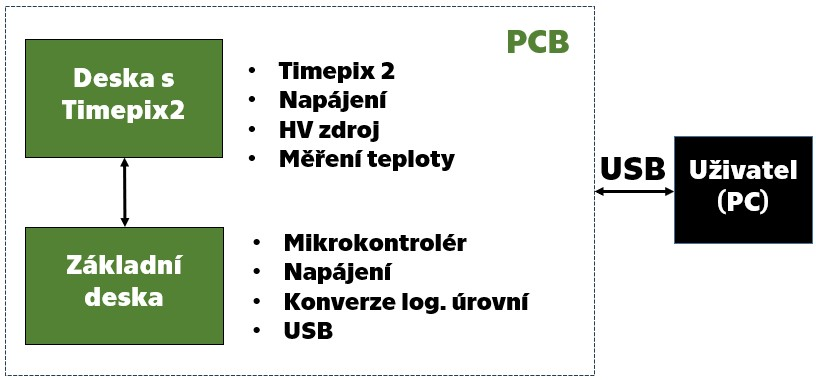
\includegraphics[scale=0.80]{navrh_reseni.jpg}
	\caption{Koncept řešení vyčítacího rozhraní pro detektor Timepix 2} 
	\label{fig:navrh_reseni}
\end{figure}

\subsection{Komunikace s Timepix 2}
Pro komunikaci s Timepix 2 je možné využít sériové, nebo paralelní rozhraní, jak již bylo zmíněno v části \ref{Komunikacni rozhrani}. Pro tuto práci uvažujme využití pouze sériové komunikace. Využití sériového rozhraní pro komunikaci s Timepix 2, umožní použít mikrokontrolér. Maximální vyčítací rychlost z detektoru Timepix 2 je 100 Mbits/s. S ohledem na tuto maximální rychlost vyčítaní dat z Timepix 2 musí být vybrán vhodný mikrokontrolér pro obsluhu komunikace, nejen s Timepix 2 detektorem. 

\subsection{Uživatelské komunikační rozhraní}
Komunikační rozhraní pro tuto práci bylo zvoleno rozhraní USB s konektorem typu C. Použit byl standart USB 2.0 High Speed. Tento standart umožňuje komunikovat maximální rychlostí až 480 Mbit/s. S respektem na maximální rychlost vyčítání dat z detektoru Timepix 2, která je 100 Mbits/s, je tato rychlost dostačující. 

\subsection{Napájení}
Pro napájení detektoru Timepix 2 jsou dle \ref{tab:tpx2_napajeni} zapotřebí tři napájecí napětí. Napájecí zdroje musí být vhodné pro maximální odběr detektoru Timepix 2. Kde uvedená celková spotřeba samotného detektoru, by neměla být dle \ref{Timepix2} vyšší než něž 900 mW. 
\par Dalším potřebným napájením potřebným pro navržený koncept je napájení mikrokontroléru. Toto napájení je závislé na konkrétním typu mikrokontroléru. Detailnější informace o výběru mikrokontroléru a jeho potřebných napájecích úrovní budou v popsány části \ref{realizace}. 

\subsection{Zapouzdření rozhraní}
Návrh rozhraní je rozložen do dvou desek plošných spojů spojenými konektorem. Při návrhu mechanické části rozhraní musí být zajištěna mechanická odolnost vůči poškození, především nejcitlivější části a to části, ve které se nachází \textit{wire bondy} propojující Timepix 2 s deskou plošných spojů \ref{fig:bga}.Dále uživatel musí být schopen se pomocí konektoru připojit k vyčítacímu rozhraní. V neposlední řadě musí být zajištěn odvod tepla ze součástek vyčítacího rozhraní, které mají největší výkon. Těmito součástky z navrženého konceptu budou především samotný detektor Timepix 2, mikrokontrolér a napájecí zdroje. 
